\documentclass[../main.tex]{subfiles}

\begin{document}
    \chapter{Плазмоны}
    
    Плазмоны - это квазичастицы, отвечающие квантованию 
    Ленгмюровских колебаний. Они в значительной мере 
    определяют оптические свойства материалов, в том числе 
    гетероструктур на основе $Hg_xCd_{1-x}Te$.
    
    \section{Дисперсионные соотношения плазмонов}

    Поскольку речь идёт о квантовании классических ЭМ колебаний, 
    для получения дисперсионного соотношения необходимо найти 
    материальные соотношения, а в частности - зависимость 
    диэлектрической проницаемости от частоты.

    Формула для поправки к диэлектрической проницаемости от 
    учёта плазмонных эффектов носит имя Линдхарда:
    \begin{equation}
        \label{lindhard}
        \kappa_{pl}(\vec q, \omega) = \frac{4\pi}{\vec{q}^2 V}
            \sum_{m, n} \int d\vec k \frac{f_m(\vec k) - f_n(\vec k 
                + \vec q)}{\varepsilon_n(\vec k + \vec q) - 
                \varepsilon_m - \hbar \omega - \i \hbar \alpha}
                \bra{\psi_{\vec k + \vec q,n}} \ket{\psi_{\vec k, m}};
    \end{equation}

    Ленгмюровские колебания являются колебаниями поляризации. Таким
    образом они должны подчиняться уравнению связи поляризации и 
    плотности свободного заряда $\div \vec P  = - \rho$. Кроме того 
    такие колебания могут возбуждаться внешним электрическим полем, 
    которое мы примем потенциальным $\vec E = - \grad \varphi$

    В общем виде функции представляются в виде огибающей, зависящей 
    от времени и быстроосциллирующего члена. В частности:
    \begin{equation}
        \label{plasmons:wf0}
        \ket{\vec k, m} = \frac{1}{\sqrt S} \exp{i\vec k \vec r}
            \exp{-i \omega_{\vec k, m} t} \psi_{\vec k, m};
    \end{equation}

    Здесь $\vec k$ - волновой вектор, которому отвечает функция, 
    $m$ - номер подзоны с учётом спина и размерного квантования 
    по оси $z$. $\psi_{\vec k, m}$ - волновые функции
    \ref{calculation:wf}, полученные по методике, 
    описанной в прошлой главе \ref{chapter:calcs}. 

    Электрическое поле в виде \ref{} должно вызывать искажения 
    такой равновесной волновой функции с волновыми векторами
    $\vec k \pm \vec q$, т.e. в первом порядке малости по полю:
    \begin{equation}
        \label{plasmons:wf1}
        \psi_m (\vec k, \vec r) = \ket{\vec k, m} + \sum_n b_{\vec k 
            + \vec q, m, n} (t) \ket{\vec k + \vec q, n} + \sum_n 
            c_{\vec k - \vec q, m, n} (t) \ket{\vec k - \vec q, n};
    \end{equation}

    В таком случае плотность заряда может быть записана как:
    \begin{multline}
        \label{charge_density}
        \rho = -e \sum_{m} \int d\vec k  \left(
            \bra{\psi_m (\vec k, \vec r}\ket{\psi_m (\vec k, 
            \vec r} - 1\right) f_m(\vec k) =
            \sum_{m, n} \int d \vec k f_m (\vec k) \\
            \left( b_{\vec k + \vec q, m, n} (t)
            \bra{\vec k, m} \ket{\vec k 
            + \vec q, n} + b^\dagger_{\vec k + \vec q, m, n} (t) 
            \bra{\vec k + \vec q, n} \ket{\vec k, m}\right.\\ 
            \left. + c_{\vec k - \vec q, m, n} (t) \bra{\vec k, m} 
            \ket{\vec k  - \vec q, n} + c^\dagger_{\vec k - \vec q, m, n} 
            (t) \bra{\vec k - \vec q, n} \ket{\vec k, m} \right);
    \end{multline}
    
    Для получения коэффициентов $b,~c$ воспользуемся нестационарной 
    теорией возмущений.

    Результатом для вычисления коэффициентов является:
    \begin{equation}
        \label{plasmons:charge:coeffs}
        \begin{aligned}
            b_{\vec k + \vec q, m, n} (t) = U \frac{\exp{-i\omega t - i 
                \varepsilon_m (\vec k) t / \hbar + i \varepsilon_n(\vec k 
                + \vec q) t / \hbar + \alpha t}}{\varepsilon_m (\vec k) + \hbar 
                \omega - \varepsilon_n(\vec k + \vec q)+ i \hbar \alpha}
                \bra{\psi_{\vec k+\vec q, n}}\ket{\psi_{\vec k, m}}; \\
            c_{\vec k - \vec q, m, n} (t) = U^\dagger \frac{\exp{i\omega t - i 
                \varepsilon_m (\vec k) t / \hbar + i \varepsilon_n(\vec k 
                - \vec q) t / \hbar + \alpha t}}{\varepsilon_m (\vec k) - \hbar 
                \omega - \varepsilon_n(\vec k - \vec q)+ i \hbar \alpha}
                \bra{\psi_{\vec k+\vec q, n}}\ket{\psi_{\vec k, m}};
        \end{aligned}
    \end{equation}

    В частности, стоит отметить, что для случая квантовой ямы, скалярное 
    произведение функций вида $\psi_{k, m}$ будет содержать в том числе 
    и скалярное произведение по оси $z$. Предполагая квантованность по 
    этой оси:
    \begin{multline}
        \bra{\psi_{\vec q, n}}\ket{\psi_{\vec k, m}} = 
            \bra{\sum_i \exp{k_{z,i} \sum_j c_{nij \vec q}} u_j(\vec r)}
            \ket{\sum_i \exp{k_{z,i} \sum_j c_{mij \vec k}} u_j(\vec r)}\\ 
            = \sum_{s=\{i,j\}}  c^\dagger_{ns \vec q} c_{ms \vec k};
    \end{multline}

    Подставляя полученные выражения в \ref{charge_density} 
    и приводя подобные можно получить:
    \begin{multline}
        \rho = \frac{e^2 U}{S} \exp{i\vec q \vec r - i \omega t + \alpha t}
            \sum_{m, n} \int d\vec k \left( \frac{\bra{\psi_{\vec k + \vec q, n}}
            \ket{\psi_{\vec k, m}}}{\varepsilon_m(\vec k) + \hbar \omega - 
            \varepsilon_n(\vec k + \vec q) + i \hbar \alpha} +\right. \\ 
            \left. \frac{\bra{\psi_{\vec k - \vec q, n}}
            \ket{\psi_{\vec k, m}}}{\varepsilon_m(\vec k) - \hbar \omega - 
            \varepsilon_n(\vec k - \vec q) - i \hbar \alpha} \right) + \text{c.c.}=\\
            \frac{e^2 U}{S} \exp{i\vec q \vec r - i \omega t + \alpha t}
            \sum_{m, n} \int d\vec k \bra{\psi_{\vec k + \vec q, n}}
            \ket{\psi_{\vec k, m}} \frac{f_m(\vec k) - f_n(\vec k - \vec q)}
            {\varepsilon_m(\vec k) + \hbar \omega - \varepsilon_n(\vec k + \vec q) 
            + i \hbar \alpha};
    \end{multline}

    Учитывая это выражение мы получаем формулу Линдхарда \ref{lindhard}. Обладая 
    этим знанием сравнительно легко получить дисперсионное соотношение для плазмонов,
    решая следующее уравнение:
    \begin{equation}
        \label{plasmons:disp}
        \frac{1}{(2\pi)^2}\frac{\kappa^2}{\kappa^2_{pl}} = 
        \vec{q}^2 - \kappa \frac{\omega^2}{c^2};
    \end{equation}
    
    Очевидно, что это уравнение может иметь мнимые корни. Причём, как правило,
    численно удобнее решать это уравнение, задавая частоту и решая относительно 
    волнового вектора.

    Также то уравнение имеет два корня, отвечающие "нижней" и "верхней" ветвям 
    дисперсионного соотношения.

    \section{Результаты расчёта спектра полазмонов}

    В дальнейшем будут показаны зонные спектры плазмонов "верхней" ветки в 
    квантовой яме толщиной $6~\text{nm}$, имеющую состав ямы $HgTe$ и 
    барьеров $CdTe$. При этом структура полагается выращенной в кристаллографическом
    направлении [013], а температура решётки и температура носителей заряда равной 
    температуре жидкого гелия $4.2~\text{K}$. Продемонстрированны срезы 
    $\vec k = (k_x, 0)$.

    \begin{figure}[h]
        \begin{minipage}[h]{0.49\textwidth}
            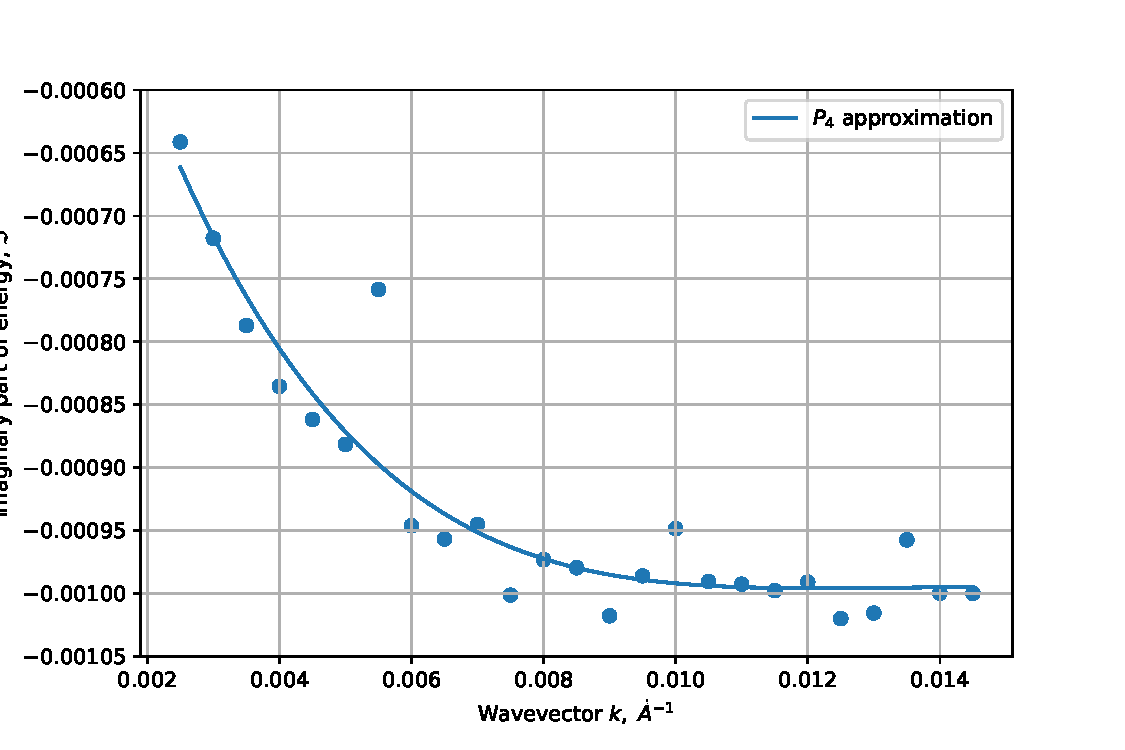
\includegraphics[width=0.9\textwidth]{./images/plasmon_6nm_25_001_im.pdf}
            \caption{Мнимая часть частоты в зависимости от волнового вектора, при $N_e = 2.5 \cdot 10^{11}~\text{cm}^{-2},~N_h = 10^9~\text{cm}^{-2}$
            \label{plasmon:6nm25ne001npim}}
        \end{minipage}
        \hfill
        \begin{minipage}[h]{0.49\textwidth}
            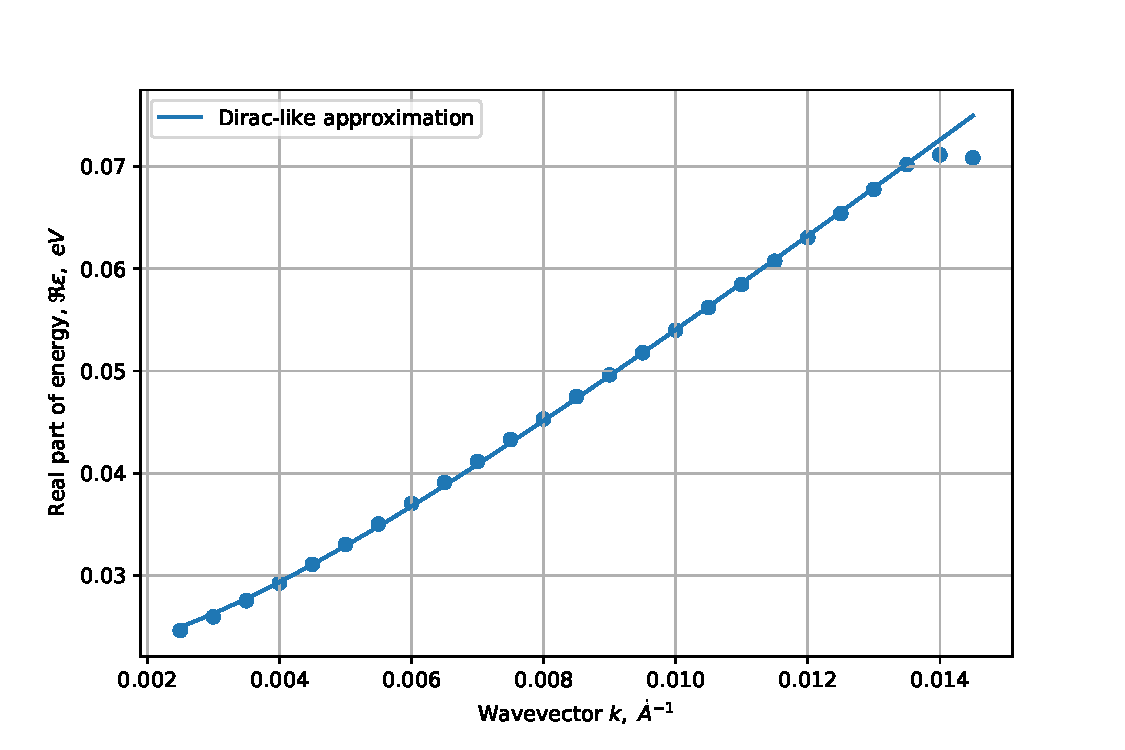
\includegraphics[width=0.9\textwidth]{./images/plasmon_6nm_25_001_re.pdf}
            \caption{Действительная часть частоты в зависимости от волнового вектора, при $N_e = 2.5 \cdot 10^{11}~\text{cm}^{-2},~N_h = 10^9~\text{cm}^{-2}$
            \label{plasmon:6nm25ne001npre}}
        \end{minipage}
    \end{figure}

    На представленных выше графиках \ref{plasmon:6nm25ne001npim}, \ref{plasmon:6nm25ne001npre} видно видно несколько особенностей.
    В частности заметно, что в данном случае плазмоны могут лишь поглощать ЭМ волны. Также видно, что мнимая часть частоты вычисляется 
    неустойчиво (т.е. "выбросы" на Рис. \ref{plasmon:6nm25ne001npim} являются артевфактами численного расчета).

    Однако при некоторых условиях плазмоны могут иметь и положительную часть частоты, что соответствует усилению ЭМ волн. Для того, 
    чтобы эти условия удовлетворялись необходимо, чтобы в полупроводнике была существенная инверсия населенности. Такие явления 
    могут наблюдаться, к примимеру, после накачки. Особый интерес представляет "граница" концентрации, при которой будет наблюдатьтся 
    усиление. Одно из таких дисперсионных соотношений приведено ниже Рис. \ref{plasmon:6nm3ne0125npim}, \ref{plasmon:6nm3ne0125npre}.

    \begin{figure}[h]
        \begin{minipage}[h]{0.49\textwidth}
            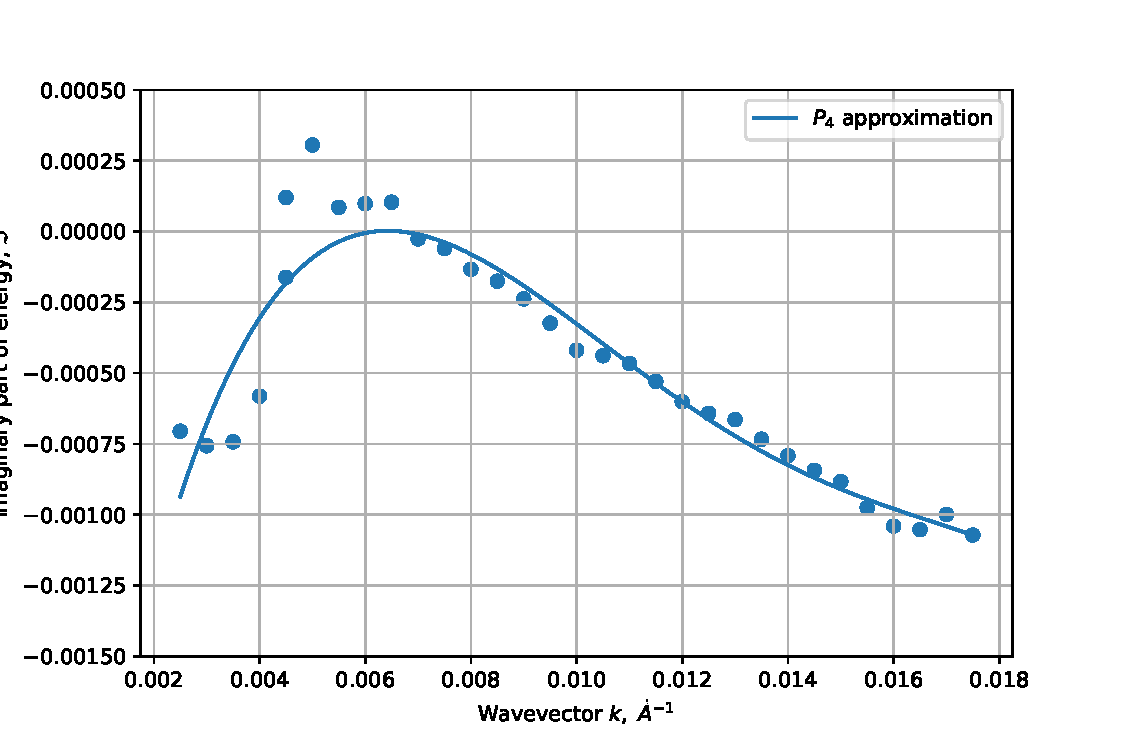
\includegraphics[width=0.9\textwidth]{./images/plasmon_6nm_3_0125_im.pdf}
            \caption{Мнимая часть частоты в зависимости от волнового вектора, при $N_e = 3 \cdot 10^{11}~\text{cm}^{-2},~N_h = 1.25 \cdot 10^{10}~\text{cm}^{-2}$
            \label{plasmon:6nm3ne0125npim}}
        \end{minipage}
        \hfill
        \begin{minipage}[h]{0.49\textwidth}
            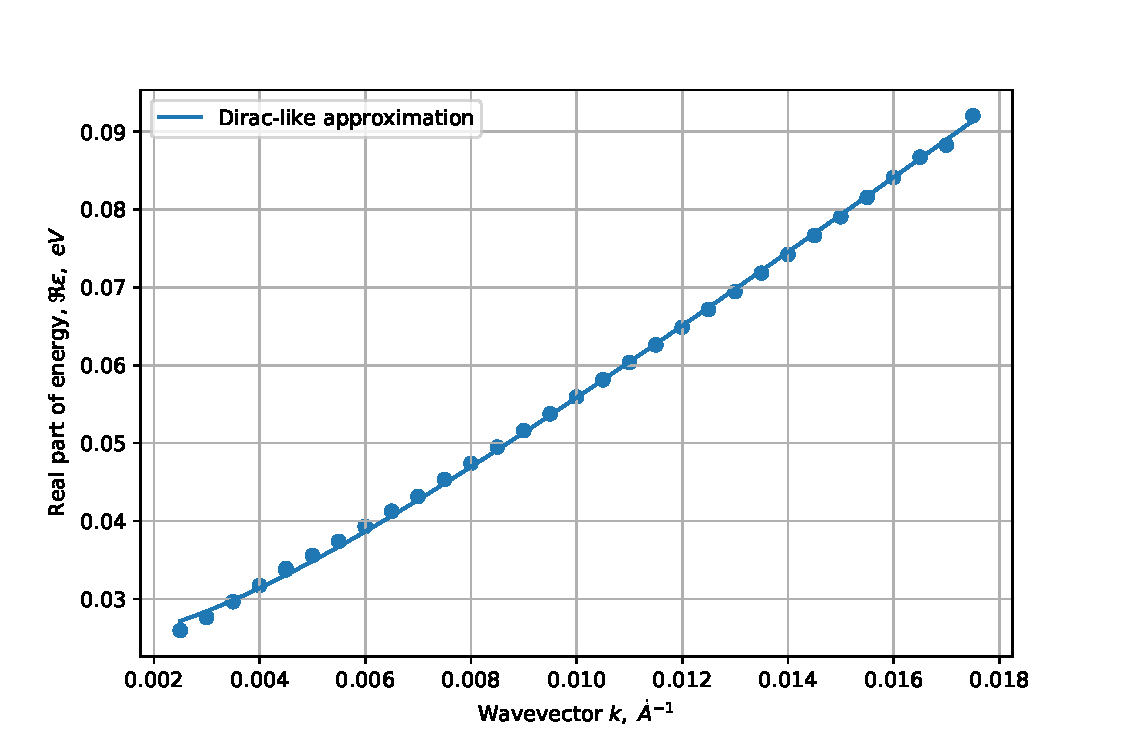
\includegraphics[width=0.9\textwidth]{./images/plasmon_6nm_3_0125_re.pdf}
            \caption{Действительная часть частоты в зависимости от волнового вектора, при $N_e = 3 \cdot 10^{11}~\text{cm}^{-2},~N_h = 1.25 \cdot 10^{10}~\text{cm}^{-2}$
            \label{plasmon:6nm3ne0125npre}}
        \end{minipage}
    \end{figure}

    Для того чтобы оценить, что действительно существует порог можно посмотреть на сводную диаграмму для семейства дисперсионных соотношений
    при постоянной концентрации электронов и изменяющейся концентрации дырок \ref{plasmon:6nm3neXnpim}.

    \begin{figure}[h]
        \begin{minipage}[h]{0.7\textwidth}
            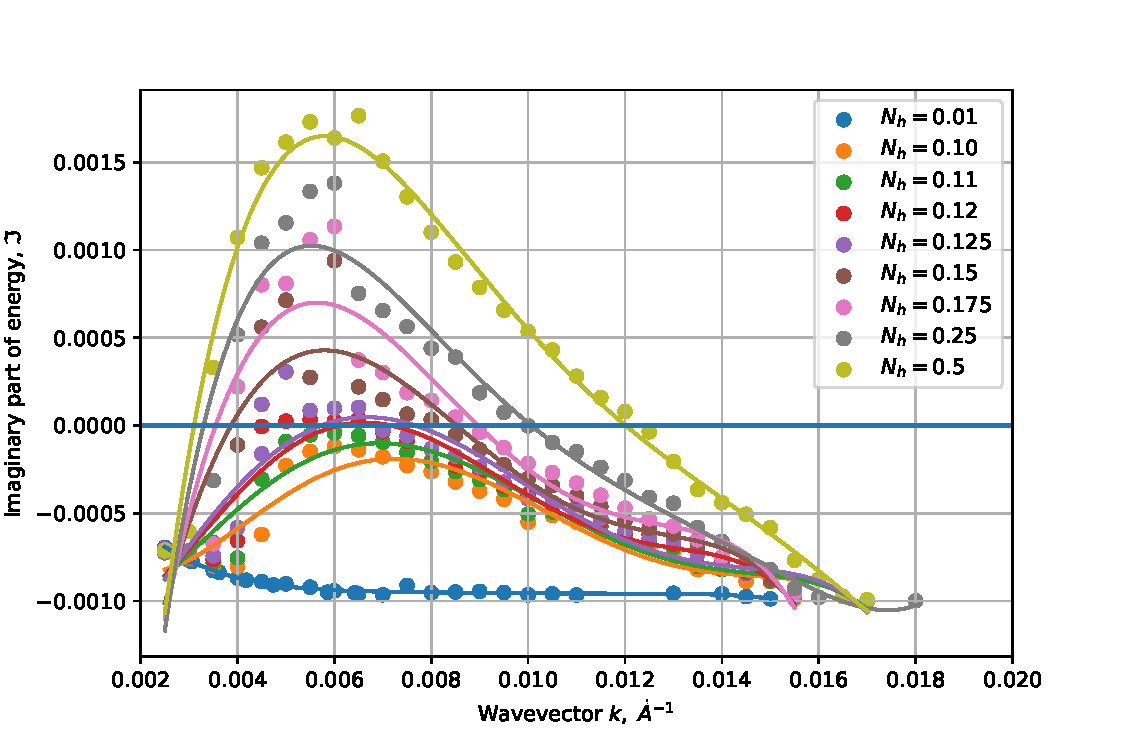
\includegraphics[width=0.9\textwidth]{./images/plazmon6nm3neXnpim.pdf.pdf}
            \caption{Мнимая часть частоты в зависимости от волнового вектора, при $N_e = 3 \cdot 10^{11}~\text{cm}^{-2},~N_h = x \cdot 10^{10}~\text{cm}^{-2}$,
            где $x$ указан на графике.\label{plasmon:6nm3neXnpim}}
        \end{minipage}
    \end{figure}
    

\end{document}